\subsubsection*{T2}

Геометрически выходит гипербола, доказываем.

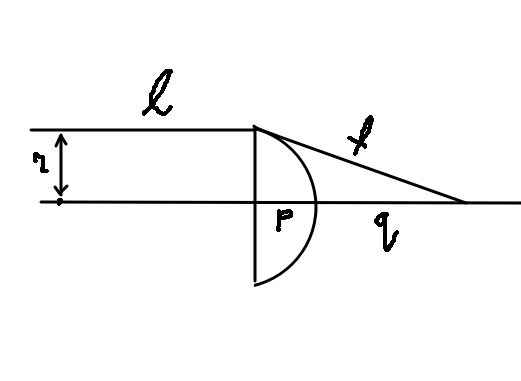
\includegraphics{parts/img/T2.png}

Так как длина оптических путей должна совпадать, то запишем равенство

\begin{equation*}
	l + f = l + np + q 
\end{equation*}

Таким образом, приходим к равенству

\begin{equation*}
	np + q = \sqrt{(p+q)^2 + r^2}
\end{equation*}

\begin{equation*}
	(n^2 - 1)p^2 + 2 p q (n -1)  = r^2
\end{equation*}
Что сводится к уравнению гиперболы в координатах $(p,r)$